\documentclass[letterpaper,11pt,oneside,reqno]{article}

%%%%%%%%%%%%%%%%%%%%%%%%%%%%%%%%%%%%%%%%%%%%%%%%%%%%%%%%%%%%

\usepackage[pdftex,backref=page,colorlinks=true,linkcolor=blue,citecolor=red]{hyperref}
\usepackage[alphabetic,nobysame]{amsrefs}

%%%%%%%%%%%%%%%%%%%%%%%%%%%%%%%%%%%%%%%%%%%%%%%%%%%%%%%%%%%%
%main packages
\usepackage{amsmath,amssymb,amsthm,amsfonts,mathtools}
\usepackage{graphicx,color}
\usepackage{upgreek}
\usepackage[mathscr]{euscript}

%equations
\allowdisplaybreaks
\numberwithin{equation}{section}
%tikz
\usepackage{tikz}

%conveniences
\usepackage{array}
\usepackage{adjustbox}
\usepackage{cleveref}
\usepackage{enumerate}
\usepackage{datetime}

%paper geometry
\usepackage[DIV=12]{typearea}

%%%%%%%%%%%%%%%%%%%%%%%%%%%%%%%%%%%%%%%%%%%%%%%%%%%%%%%%%%%%
%draft-specific
\synctex=1
% \usepackage{refcheck,comment}

%%%%%%%%%%%%%%%%%%%%%%%%%%%%%%%%%%%%%%%%%%%%%%%%%%%%%%%%%%%%
%this paper specific
\newcommand{\ssp}{\hspace{1pt}}

%%%%%%%%%%%%%%%%%%%%%%%%%%%%%%%%%%%%%%%%%%%%%%%%%%%%%%%%%%%%
\newtheorem{proposition}{Proposition}[section]
\newtheorem{lemma}[proposition]{Lemma}
\newtheorem{corollary}[proposition]{Corollary}
\newtheorem{theorem}[proposition]{Theorem}
%%%%%%%%%%%%%%%%%%%%%%%%%%%%%%%%%%%%%%%%%%%%%%%%%%%%%%%%%%%%
\theoremstyle{definition}
\newtheorem{definition}[proposition]{Definition}
\newtheorem{remark}[proposition]{Remark}
\newtheorem{example}[proposition]{Example}
%%%%%%%%%%%%%%%%%%%%%%%%%%%%%%%%%%%%%%%%%%%%%%%%%%%%%%%%%%%%
\theoremstyle{remark}
\newtheorem{exercise}{Exercise}[section]

\begin{document}
\title{How to Solve the Stochastic Six Vertex Model}

% OTHER AUTHORS 

% \author{Matthew Nicoletti and Leonid Petrov}
\author{Leonid Petrov}

\date{At \currenttime{}, on \today}

\setcounter{tocdepth}{4}

\maketitle


\section*{Introduction}

These are lecture notes for \href{https://www.math.tamu.edu/conferences/functional_analysis/PANEM.html}{\texttt{PANEM-2023}} at Texas A{}\&M on the integrability and asymptotics of the stochastic six vertex model.



\newpage
\section{Lecture I. Six vertex model through different lenses}
\label{sec:6v_model_lecture}

In the first lecture, we describe the stochastic six vertex model
from two diverse perspectives --- as a model of statistical mechanics,
and as a stochastic particle system.

\subsection{Gibbs measures and the six vertex model}
\label{sub:gibbs_6v}

\subsubsection{Finite-volume Gibbs measures}

We begin with describing the useful framework of \emph{Gibbs measures}.
For simplicity, we work on the two-dimensional lattice $\mathbb{Z}^2$.
Let $\Lambda\subset\mathbb{Z}^{2}$ be a finite subset (for example, a rectangle).
We are interested in \emph{spin configurations} inside $\Lambda$
which are encoded as $\omega=\{\sigma_e\colon e \textnormal{ is an edge in $\Lambda$}\}$,
where $\sigma_e\in\left\{ 0,1 \right\}$.
By an ``edge in $\Lambda$'' we mean that both endpoints of this edge must be inside $\Lambda$.
Each spin configuration is equipped with boundary conditions,
which are fixed spins on all the boundary edges of $\Lambda$
(an edge is called boundary if it connects $\Lambda$ to $\mathbb{Z}^{2}\setminus \Lambda$).

With each spin configuration $\omega$, we associate 
its energy
$H(\omega)\in \mathbb{R}$.
This energy
may depend on global parameters
(e.g., inverse temperature)
and local parameters (e.g., edge capacities or vertex rapidities).
If a particular spin configuration $\omega$ is forbidden, we have $H(\omega)=+\infty$.

\begin{definition}
	\label{def:Gibbs_measure_finite}
	The (finite-volume) \emph{Gibbs measure}
	in $\Lambda$ 
	with fixed boundary conditions 
	and the energy function $H(\cdot)$
	is the probability distribution on spin configurations 
	whose probability weights have the form
	\begin{equation*}
		\mathop{\mathrm{{Prob}}}(\omega)=\frac{1}{Z}\ssp\exp\left\{ -H(\omega) \right\}.
	\end{equation*}
	Here $Z$ is the \emph{partition function}, which is simply the probability normalizing constant.
\end{definition}
For a given finite region, boundary conditions, and the energy function, a 
Gibbs measure is unique.

\begin{example}[Domino tilings on the square grid]
	\label{example:dominos}
	A \emph{perfect matching} on $\Lambda$ is any subset $M$ of its edges 
	such that every vertex is covered by exactly one 
	edge from $M$.
	For example, here is a perfect matching on the four by four rectangle:
	\begin{equation*}
		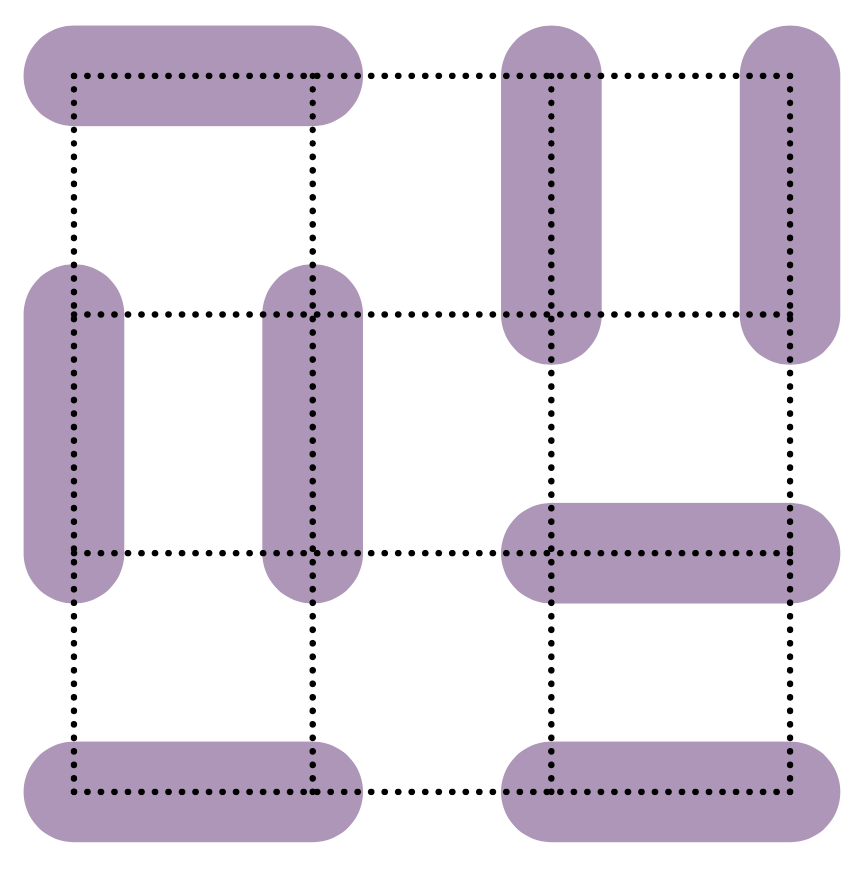
\includegraphics[width=.2\textwidth]{./images/domino_4_4.png}
	\end{equation*}
	If the set of allowed spin configurations is the 
	set of perfect matchings (with $\sigma_e=1$ if the edge is included in the matching, and 
	$\sigma_e=0$ otherwise),
	and 
	\begin{equation*}
		H(\omega)=\begin{cases}
			0,&\textnormal{$\omega$ is a perfect matching};\\
			+\infty,&\textnormal{$\omega$ is not a perfect matching},
		\end{cases}
	\end{equation*}
	then the corresponding Gibbs measure
	is the 
	uniform distribution
	on the space of \emph{domino tilings}.
	That is, we identify each covered edge with a $2\times 1$ domino.
	The domino tiling corresponding to the above perfect matching is
	\begin{equation*}
		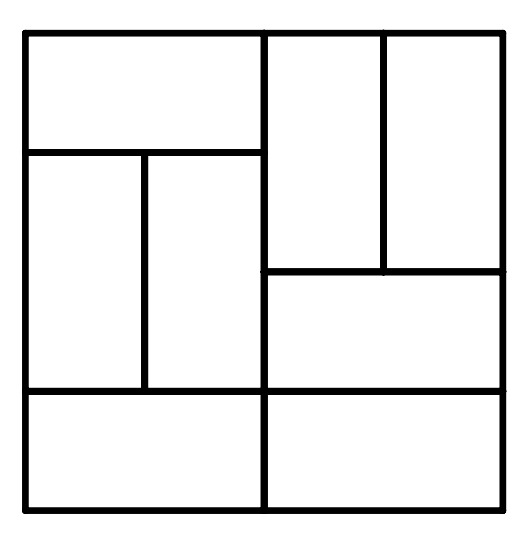
\includegraphics[width=.2\textwidth]{./images/tiling_4_4.png}
	\end{equation*}
\end{example}

\begin{exercise}
	Compute the number of domino tilings
	of the thin rectangles 
	\begin{enumerate}[(a)]
		\item $2\times n$;
		\item $3\times (2n)$.
	\end{enumerate}
\end{exercise}

Computing partition functions of various Gibbs measures
may be challenging. For example, the number of 
domino tilings of the $8\times 8$ chessboard is 12,988,816,
but its theoretical computation (not via a computer program)
requires several nontrivial steps \cite{Kasteleyn1961}, \cite{temperley1961dimer}. 

Parameter-dependent partition functions represent many important 
quantities across all of mathematics, including various
families of symmetric functions (such as Schur or Hall-Littlewood functions), and related objects.

\subsubsection{Infinite-volume Gibbs measures}

Besides Gibbs measures on configurations on a
finite space as in \Cref{def:Gibbs_measure_finite} with fixed boundary
conditions (``\emph{boxed distributions}''), we are 
interested
in \emph{infinite-volume} Gibbs measures. 

\begin{definition}
	\label{def:infinite_Gibbs}
	A probability measure on spin configurations on 
	an infinite subset $\Lambda_\infty\subseteq\mathbb{Z}^{2}$
	(we will mainly consider the whole plane and the quarter plane $\mathbb{Z}_{\ge0}^{2}$)
	is called (infinite-volume) Gibbs if for any finite $\Lambda\subset \Lambda_\infty$,
	the configuration inside $\Lambda$
	conditioned on the configuration in $\Lambda_\infty\setminus \Lambda$
	is a finite-volume Gibbs measure in the sense of \Cref{def:Gibbs_measure_finite}
	(with boundary conditions imposed by the outside configuration in $\Lambda_\infty\setminus \Lambda$).
\end{definition}

Out of all possible infinite-volume Gibbs measures, we are interested in measures with 
special properties, such as translation invariant and/or ergodic.
A Gibbs measure on $\mathbb{Z}^{2}$ is called \emph{translation invariant}
if its distribution does not change under arbitrary
space translations. 
A Gibbs measure is called \emph{ergodic} (equivalently, \emph{extremal})
if it cannot be represented as a convex combination of 
two other such measures.
Gibbs measures which are translation invariant
and ergodic (within the class of translation invariant measures)
are called \emph{pure states}.

Classifying pure states for a given energy function $H(\cdot)$ is a very
nontrivial problem, and an 
explicit answer is rarely available. 
For the general six vertex model 
(defined in \Cref{subsub:6v_model} below),
the answer is only conjectural
\cite{reshetikhin2010lectures}.

On the other hand, pure states of the six vertex model 
under a special
\emph{free fermion condition}
(which includes the domino model from \Cref{example:dominos})
admit a very explicit description through
determinantal point processes 
(i.e., all correlation functions
of these measures are diagonal minors
of an explicit function in two variables),
which follows from
\cite{Sheffield2008}, 
\cite{KOS2006}.
One of the goals of these lecture notes is to discuss 
the tools and results one would require to extend this classification
beyond the free fermion case.


\begin{remark}
	\label{rmk:inf_Gibbs}
	Certain families of 
	non translation invariant
	infinite-volume
	Gibbs measures (under the free fermion condition)
	power the
	classification of irreducible representations of
	infinite-dimensional unitary group
	and other classical groups
	\cite{Voiculescu1976},
	\cite{VK82CharactersU},
	\cite{BorodinOlsh2011GT},
	\cite{Petrov2012GT}.
	This subject is closely related to symmetric
	functions arising as partition functions
	of Gibbs measures with 
	varying parameters (rapidities)
	along one of the lattice coordinate
	direction which we discuss in the second lecture (\Cref{sec:integrability}).
	There is also a direct link between these Gibbs measures and totally nonnegative triangular or
	full Toeplitz matrices for characters of the infinite
	symmetric group or, respectively, the
	infinite-dimensional unitary group, see \cite{AESW51},
	\cite{Edrei53}, \cite{Boyer1983}.
\end{remark}

\subsubsection{Six vertex model}
\label{subsub:6v_model}

The most general Gibbs property we consider in these notes is that of the 
\emph{asymmetric six vertex model}. 
The six vertex model 
was introduced by Pauling to model
the residual entropy of ice \cite{pauling1935structure}
(see also 
\cite{Nature_square_ice}
for recent experiments
with square ice between two graphene sheets, and \Cref{rmk:ice} below for an exact connection).
The model
has received a lot of attention since the seminal Bethe Ansatz solutions obtained in the 1960's in
\cite{Lieb1967SixVertex}, \cite{YangYang1966}.
We refer to the book 
\cite{baxter2007exactly} for an introduction, and also to
\cite{reshetikhin2010lectures}, \cite{BramwellHarris2020} for recent surveys of the 
model and its history, respectively.

Under the asymmetric six vertex model, 
the allowed spin configurations on the two-dimensional lattice 
are such that locally around each vertex there can be one of the following six configurations:
\begin{equation*}
	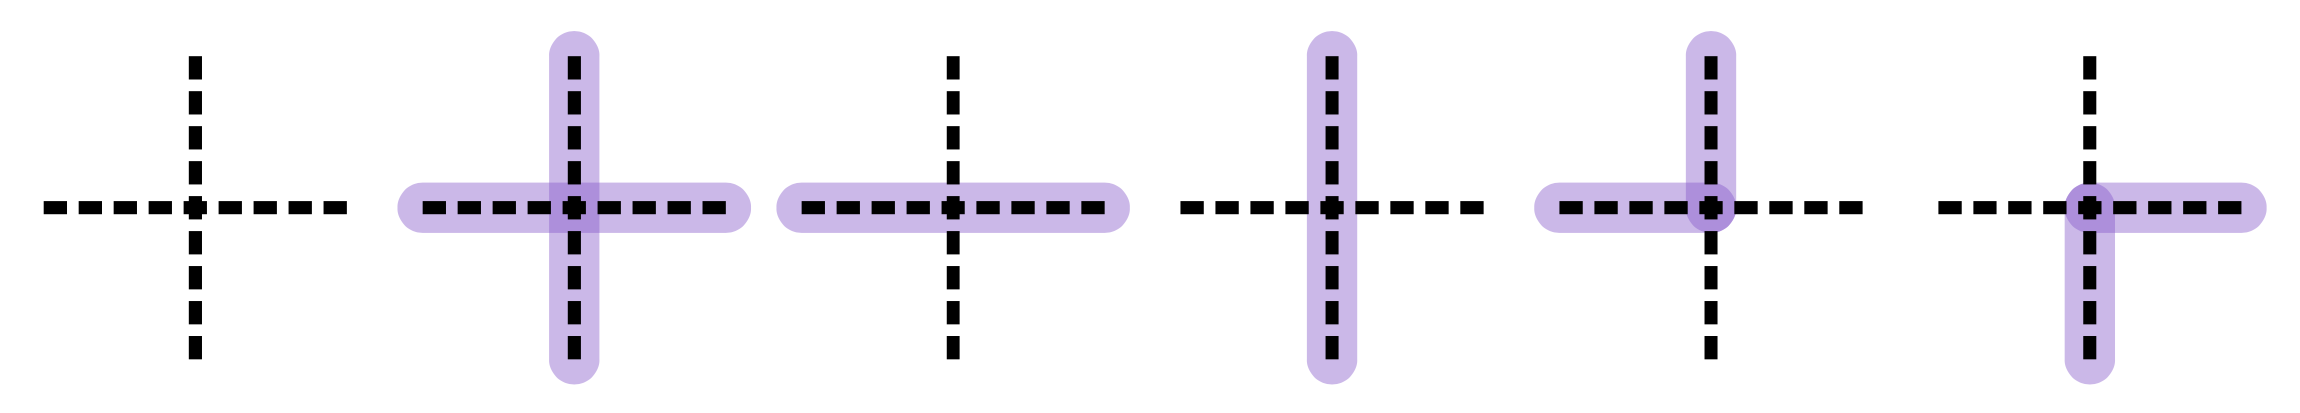
\includegraphics[width=.7\textwidth]{./images/6v_def.png}
\end{equation*}
Viewing the edges with spin $\sigma_e=1$
as parts of up-right paths, we can think of six vertex model
configurations as up-right path configurations on the lattice, where paths are allowed to touch at a
vertex.
We denote the six vertex types by $a_1,a_2,b_1,b_2,c_1,c_2$:
\begin{equation}
	\label{eq:6v_weights_picture}
	\parbox{.7\textwidth}{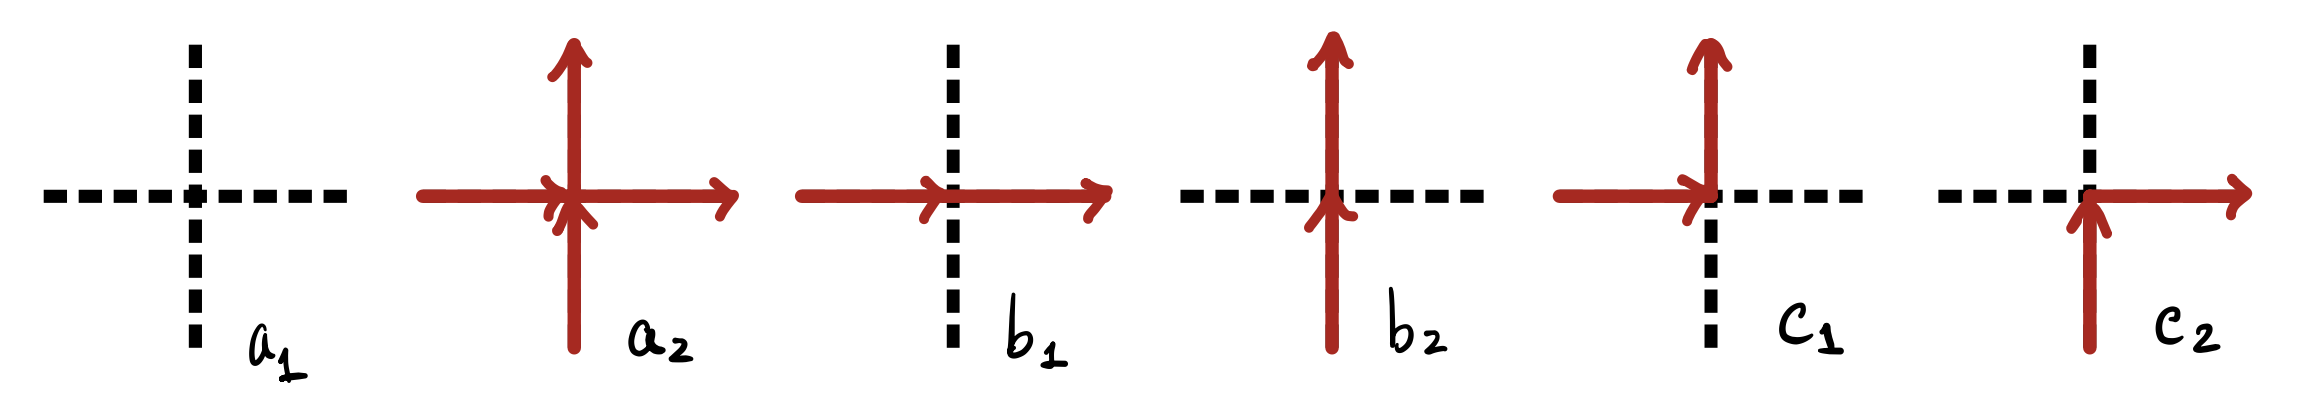
\includegraphics[width=.7\textwidth]{./images/6v_def1.png}}
\end{equation}
See \Cref{fig:ice}, right,
for an example of a global configuration of up-right paths in a rectangle.

Abusing the notation, we also think of 
$a_1,a_2,b_1,b_2,c_1,c_2\ge0$ as the Gibbs weights $e^{-H}$
assigned to each local vertex. That is, the six vertex model Gibbs measure
in a rectangle $\Lambda$ with given boundary conditions 
(that is, with prescribed spin configurations at all edges connecting
$\Lambda$ to $\mathbb{Z}^{2}\setminus\Lambda$)
has probability weights
\begin{equation*}
	\mathop{\mathrm{Prob}}(\omega)=\frac{
		a_1^{\#\{a_1\text{ vertices}\}}
		a_2^{\#\{a_2\text{ vertices}\}}
		b_1^{\#\{b_1\text{ vertices}\}}
		b_2^{\#\{b_2\text{ vertices}\}}
		c_1^{\#\{c_1\text{ vertices}\}}
		c_2^{\#\{c_2\text{ vertices}\}}
	}{Z(a_1,a_2,b_1,b_2,c_1,c_2)}.
\end{equation*}
Here 
$\#\{a_1\text{ vertices}\}$ is the number of 
vertices of type $a_1$ in the configuration $\omega$, and so on.

\begin{remark}[Connection to square ice]
	\label{rmk:ice}
	In the square ice, the oxygen atoms should 
	form a perfect square grid, and each 
	edge contains a hydrogen atom.
	The hydrogen atom on an edge is connected to one of the adjacent oxygens 
	by the chemical bond, and to another oxygen by a weaker hydrogen
	bond. 
	This allows to distinguish two types of edges, and assign
	``spins'' $0$ and $1$ to them. 
	Since each oxygen must have exactly two hydrogen
	atoms attached to it by chemical bonds, we get 
	six possible local configurations around a vertex. See \Cref{fig:ice}
	for an illustration.

	\begin{figure}[htpb]
		\centering
		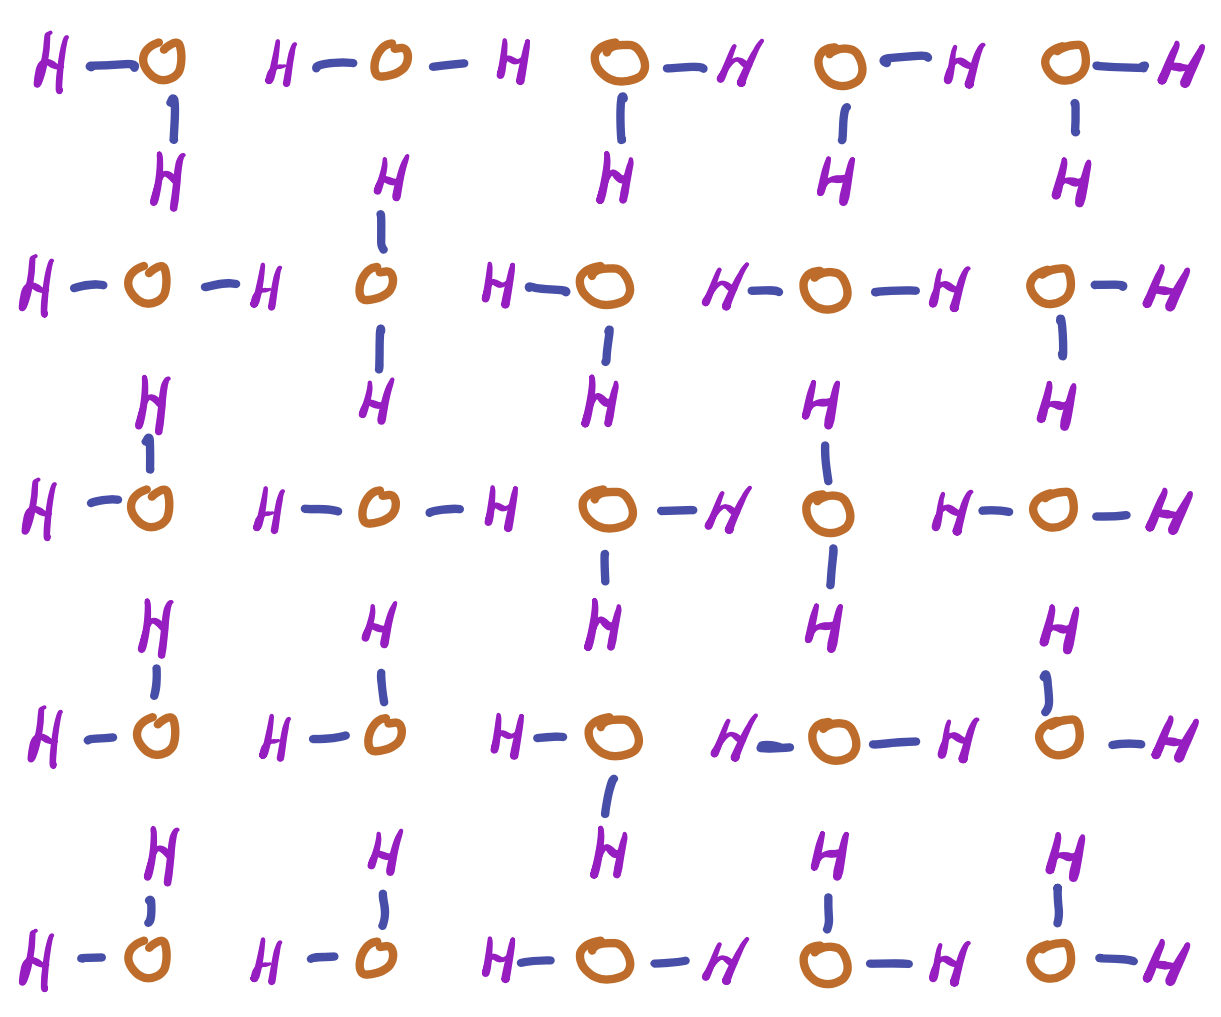
\includegraphics[width=.3\textwidth]{./images/ice.png}
		\qquad 
		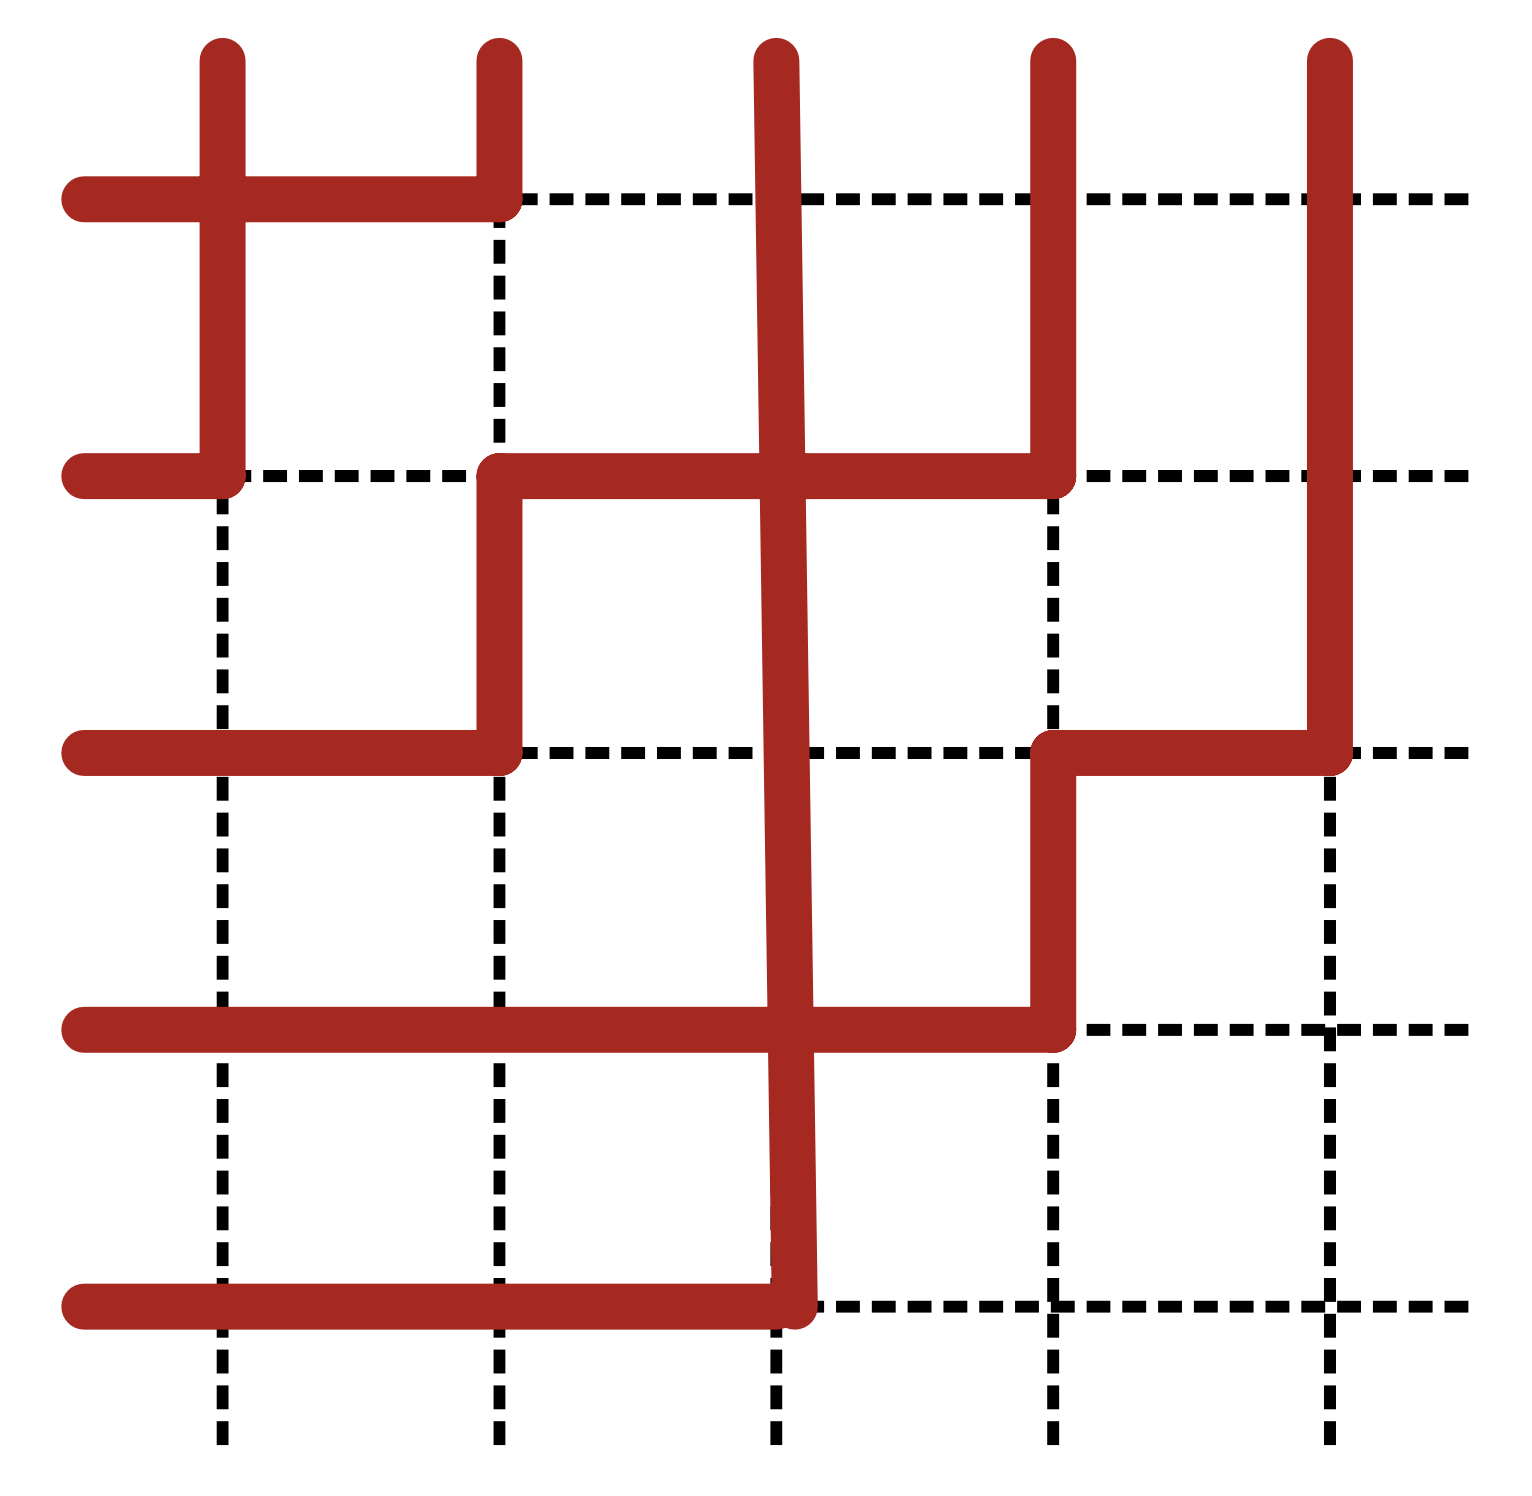
\includegraphics[width=.265\textwidth]{./images/paths.png}
		\caption{Left: a configuration of the square ice. Right:
		the corresponding configuration of the six vertex model in the square grid.}
		\label{fig:ice}
	\end{figure}
\end{remark}

The quantity
\begin{equation}
	\label{eq:delta_6v_general}
	\Delta\coloneqq \frac{a_1a_2+b_1b_2-c_1c_2}{2\sqrt{a_1a_2b_1b_2}}
\end{equation}
plays an important role in the (mostly conjectural) description
of pure phases of the asymmetric six vertex model.
Depending on $\Delta$, there are several regimes of the model:
\begin{enumerate}[$\bullet$]
	\item Ferroelectric: $\Delta>1$;
	\item Anti-ferroelectric: $\Delta<1$;
	\item Disordered: $-1<\Delta<1$;
	\item Free fermion point: $\Delta=0$.
\end{enumerate}

\begin{example}
	[Free fermion specializations]
	\label{example:free_fermion}
	Specializing the weights $a_1,a_2,b_1,b_2,c_1,c_2$ in two different free fermion ways, 
	we obtain the following particular cases:
	\begin{enumerate}[$\bullet$]
		\item If $a_1=a_2=b_1=b_2=1$ and $c_1=c_2=\sqrt 2$, 
			one can map
			six vertex configurations into domino tilings from \Cref{example:dominos}.
			This map is not a bijection between configurations, but instead 
			it splits a $c$-type vertex into two equivalent 
			local configurations of the domino tilings, while preserving the 
			configuration weights.
			This idea goes back to 
			\cite{elkies1992alternating},
			see also \cite{zinn2000six}, \cite{ferrari2006domino}.
			A multiparameter generalization of the domino tiling model
			coming from the free fermion six vertex model 
			was considered in \cite{ABPW2021free},
			see also \cite{Naprienko2023}.
		\item When $a_2=0$ and $a_1=b_1=b_2=c_1=c_2=1$,
			we forbid the intersection of paths. This model can be bijectively mapped into
			a model of \emph{lozenge tilings} (e.g., see \cite{gorin2021lectures} for the definition), 
			with configurations like
			\begin{equation*}
				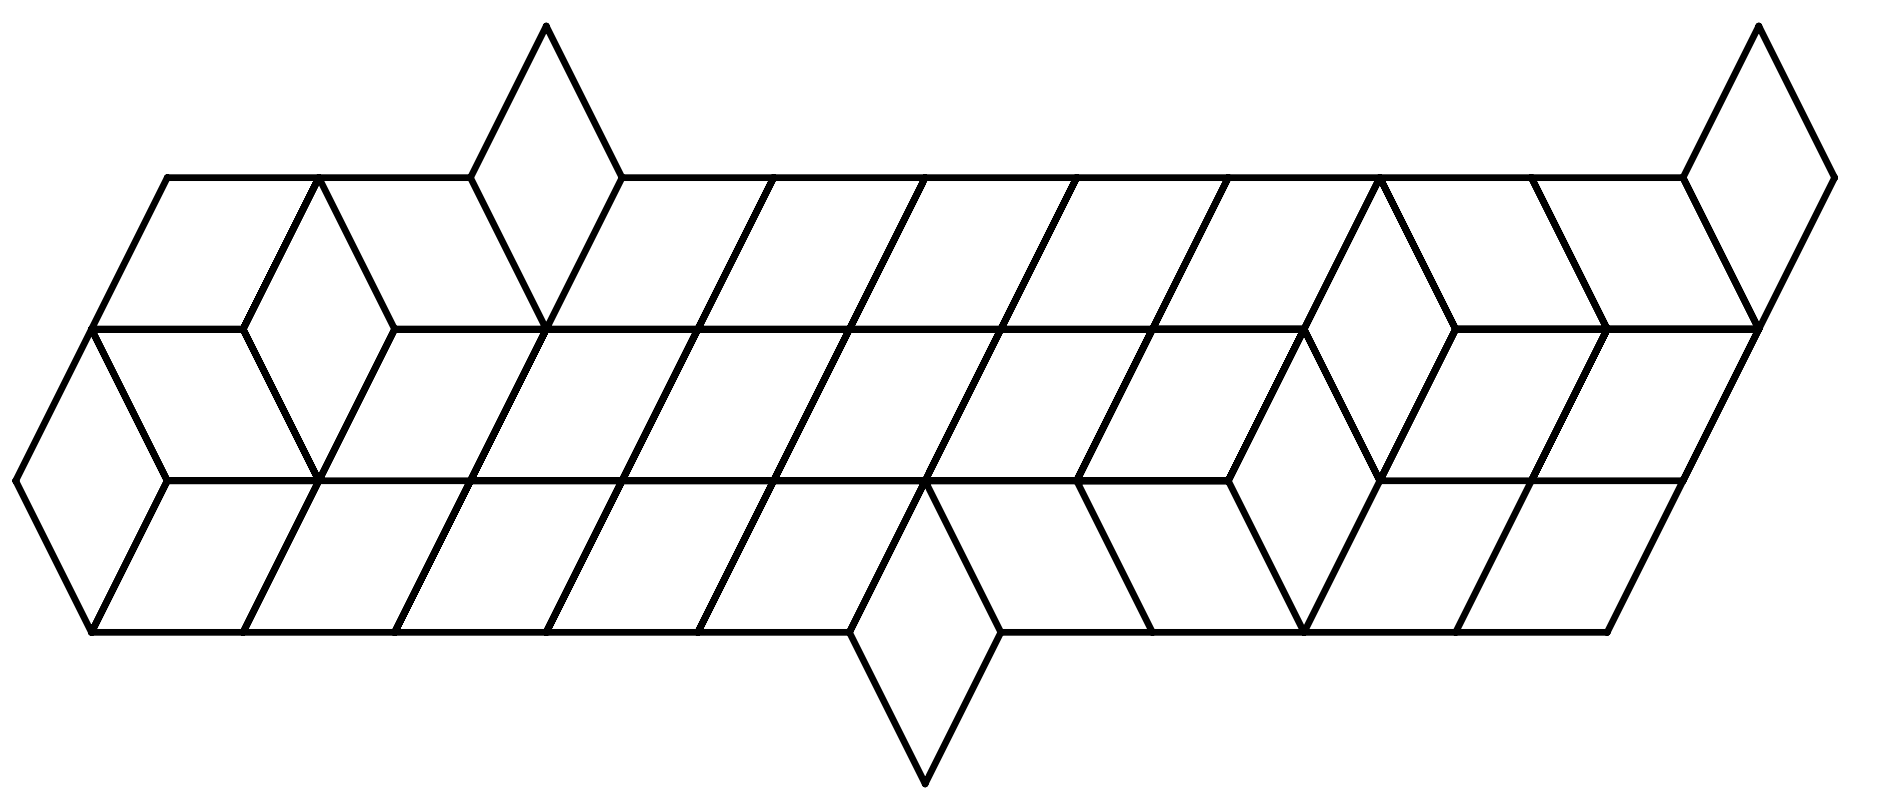
\includegraphics[width=.4\textwidth]{./images/lozenge_from_vertex.png}
			\end{equation*}
	\end{enumerate}
\end{example}

\begin{exercise}
	\begin{enumerate}[(a)]
		\item 
	Work out the details of the mapping from the 
	free fermion six vertex model with 
	$a_2=0$ and $a_1=b_1=b_2=c_1=c_2=1$ 
	to lozenge tilings. What happens to the boundary conditions?

\item
	If we set $b_1=c_1=u_xv_y$, where $(x,y)$ are the lattice coordinates of a vertex,
	then six vertex configurations
	start depending on the parameters $u_i,v_j$ (which we assume to be generic complex numbers).
	How do these weights translate into the lozenge tiling picture?
	\end{enumerate}
\end{exercise}

In the next 
\Cref{sub:s6v_and_degenerations} 
we consider another important particular case --- the 
\emph{stochastic six vertex model}, which is no longer free fermion.

\begin{remark}[Alternating sign matrices]
	There are other very interesting specializations
	of the six vertex model 
	which are not stochastic
	nor free fermion. Let us only mention
	that when $a_1=a_2=b_1=b_2=c_1=c_2=1$ (so $\Delta=1/2$, which is in the disordered regime),
	the six vertex Gibbs property becomes uniform
	(on configurations of up-right paths which are allowed to touch at a vertex).
	There is a bijection from six vertex configurations to 
	\emph{alternating sign matrices}. 
	This bijection allowed to compute the number of alternating sign matrices
	from a partition functions of the six vertex model.
	We refer to 
	\cite{kuperberg1996another} and
	\cite{Propp2001} for details.
\end{remark}

\subsection{Stochastic six vertex model and its particle system limits}
\label{sub:s6v_and_degenerations}

\subsubsection{Stochastic six vertex model}

Sampling six vertex configurations 
by Glauber dynamics (which proceeds by random local flips as in \eqref{eq:Glauber_flips} below)
can be exponentially slow under some conditions on the parameters
\cite{FahrbachRandall2019}.
Here we consider a case of parameters 
under which the sampling 
(in the case when the top and the right boundaries are ``free'')
can instead be done by running a Markov chain just once.

\begin{definition}
	\label{def:s6v}
	The six vertex model with parameters $a_1,a_2,b_1,b_2,c_1,c_2$ 
	\eqref{eq:6v_weights_picture}
	is called \emph{stochastic}
	if 
	\begin{equation}
		\label{eq:s6v_condition}
		a_1=a_2=1,\qquad 
		b_1+c_1=b_2+c_2=1,\qquad 
		b_1,b_2\in[0,1].
	\end{equation}
	The stochastic six vertex model depends on the 
	two remaining parameters
	$(b_1,b_2)$.
\end{definition}

Let us explain how conditions \eqref{eq:s6v_condition}
simplify the sampling of the model.
Take a finite rectangle $\Lambda\subset\mathbb{Z}^{2}$,
and equip it with 
\emph{free outgoing boundary conditions},
for which the locations of 
outgoing paths on the right and the top boundaries of the rectangle
are not specified. 
Due to the 
stochasticity condition \eqref{eq:s6v_condition},
the partition function of the stochastic six vertex Gibbs measure 
in $\Lambda$ with these boundary conditions is simply equal to $1$.

The stochastic six vertex configuration in $\Lambda$
can be sampled by running a row-to-row Markov chain
based on the vertex weights,
see \Cref{fig:P_u_free} for an illustration.


\begin{figure}[htpb]
	\centering
	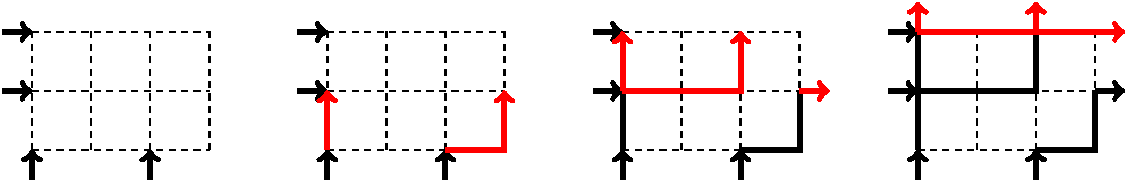
\includegraphics[width=\textwidth]{./images/fig_P_u_free.pdf}
	\caption{Sampling the configuration of the stochastic six vertex model
		in a rectangle $\Lambda$ with free outgoing boundary conditions
		by the row-to-row Markov chain. At each step, 
		we perform the sequential update (from left to right)
		in a single row using 
		the incoming paths from the left and from the row below.
		For example, after one step the probability
		of getting the displayed configuration is
		equal to 
		$b_2c_2c_1$.}
	\label{fig:P_u_free}
\end{figure}

\medskip

The stochastic six vertex model was introduced in \cite{GwaSpohn1992}.
The stochastic specialization of the parameters allows to study this particular case of the 
six vertex
model using the toolbox from stochastic interacting particle systems
\cite{Liggett1985}, by treating the vertical direction as time.
In \Cref{subsub:diagonal_limit_ASEP,subsub:PushTASEP_limit}
below we consider two limits 
of the stochastic six vertex model to 
more familiar continuous time interacting particle systems.

\subsubsection{Limit shape}
\label{subsub:limit_shape_BCG}

We are now in a position to formulate the limit shape result
for the 
stochastic six vertex model whose proof will be given in \Cref{sec:asymptotics}
in the last lecture. 
This limit shape result was first proven in \cite{BCG6V}
by adapting the techniques from the ASEP (Asymmetric Simple Exclusion Process)
pioneered in
\cite{TW_ASEP1}, \cite{TW_ASEP2}. Our goal in these lecture notes is to 
present another proof which highlights the use of several other integrability techniques,
most importantly, the Yang--Baxter equation and symmetric functions (discussed in the second lecture, \Cref{sec:integrability}).

Consider the stochastic six vertex model 
in the quadrant $\mathbb{Z}_{\ge0}^{2}$
with 
the \emph{infinite domain wall}
boundary conditions. That is, there are incoming arrows at each edge along the left 
boundary of the quadrant, and no incoming arrows at the bottom boundary.

The stochastic six vertex model in this infinite domain
can be sampled by running a Markov chain as in \Cref{fig:P_u_free}.
See \Cref{fig:CS6V}, right, for an example of a configuration.

Define the height function of the vertex model at the discrete level
by
\begin{equation}
	\label{eq:height_function}
	H(x,y)\coloneqq \#\{\textnormal{up-right paths to the right of the point $(x,y)$} \},
	\qquad (x,y)\in \mathbb{Z}_{\ge0}^2.
\end{equation}
See
\Cref{fig:s6v_height_function}
for an example.

\begin{figure}[htpb]
	\centering
	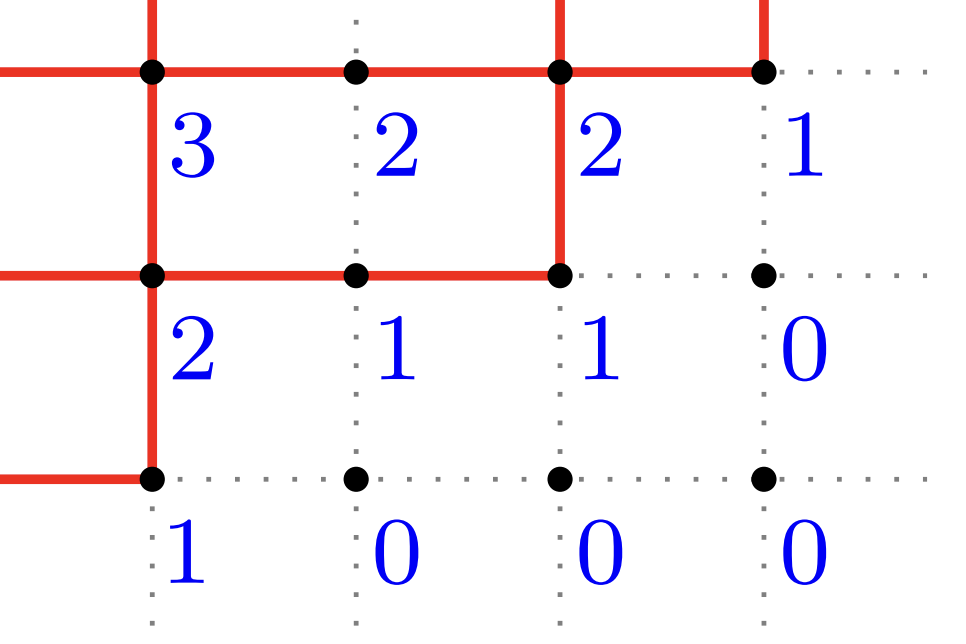
\includegraphics[width=.3\textwidth]{./images/s6v_height_function.png}
	\caption{Height function of the stochastic six vertex model with infinite domain wall
	boundary conditions.}
	\label{fig:s6v_height_function}
\end{figure}

Let $b_1>b_2$ and
\begin{equation}
	\label{eq:u_spectral_parameter}
	u\coloneqq \frac{1-b_1}{1-b_2}.
\end{equation}
Define the following function on $\mathbb{R}_{\ge0}^{2}$:
\begin{equation}
	\label{eq:limit_shape_height_function}
	\mathfrak{h}(\mathsf{x},\mathsf{y})\coloneqq
	\begin{cases}
		\mathsf{y}-\mathsf{x},
		& \text{if } \frac{\mathsf{y}}{\mathsf{x}} > \frac{1}{u} ;\\
		\dfrac{(\sqrt{\mathsf{y}} - \sqrt{u \mathsf{x}})^2}{1 - u}, & \text{if } u < \frac{\mathsf{y}}{\mathsf{x}} < \frac{1}{u}; \\
		0,&
		\text{if } \frac{\mathsf{y}}{\mathsf{x}} < u.
	\end{cases}
\end{equation}

\begin{theorem}[Limit shape of the stochastic six vertex model \cite{BCG6V}]
	\label{thm:BCG6V_limit_shape}
	We have convergence in probability for any $(\mathsf{x},\mathsf{y})\in \mathbb{R}_{\ge0}^2$:
	\begin{equation*}
		\lim_{\varepsilon\to 0}
		\ssp \varepsilon\ssp
		H\left( 
		\lfloor \varepsilon^{-1}\mathsf{x} \rfloor ,
		\lfloor \varepsilon^{-1}\mathsf{y} \rfloor \right)
		=\mathfrak{h}(\mathsf{x},\mathsf{y}),
	\end{equation*}
	where the limiting height function $\mathfrak{h}$ is given by \eqref{eq:limit_shape_height_function}.
\end{theorem}

The condition $b_1>b_2$ in \Cref{thm:BCG6V_limit_shape} is important, as for $b_1\le b_2$
the up-right paths will not travel macroscopically far to the right, and the limit shape 
function is simply $y-x$ when $y>x$. 
In the symmetric case $b_1=b_2$, there should be a limit shape result on the scale $\varepsilon^{-1/2}$ instead of
$\varepsilon^{-1}$ (for example, see \cite{ImamuraMallickSasamoto2021} and references therein to related work).

\begin{remark}
	\label{rmk:fluctuations}
	Along with \Cref{thm:BCG6V_limit_shape}, we will
	show that the fluctuations of the height function
	$H$ around its limit 
	$\mathfrak{h}$ have order $\varepsilon^{-1/3}$,
	and are given by the GUE Tracy--Widom distribution $F_2$.
	This was also obtained in \cite{BCG6V}.
	The GUE Tracy--Widom fluctuations were first observed 
	in random matrix theory
	\cite{Forrester1993},
	\cite{tracy_widom1994level_airy}.
	For the stochastic six vertex model, 
	these fluctuations manifest the fact that the
	model belongs to the \emph{KPZ universality class}
	named after the seminal work of 
	Kardar--Parisi--Zhang \cite{KPZ1986}.
	See, for example, \cite{CorwinKPZ}
	for a survey on KPZ universality.
\end{remark}

\subsubsection{Diagonal limit to ASEP}
\label{subsub:diagonal_limit_ASEP}

Let us take the limit of the stochastic six vertex model 
with the infinite domain wall boundary condition 
as $b_1,b_2\to0$, but their ratio $b_2/b_1=q$ stays fixed.
When $b_1=b_2=0$,
each up-right path performs a deterministic staircase motion. 
However, in the limit as $b_1,b_2\to0$,
as we take a large domain of the size proportional to $b_2^{-1}$, the staircases
will occasionally move ``up'' or ``down''.
More precisely, let us view the diagonal direction as the new time axis:
\begin{equation*}
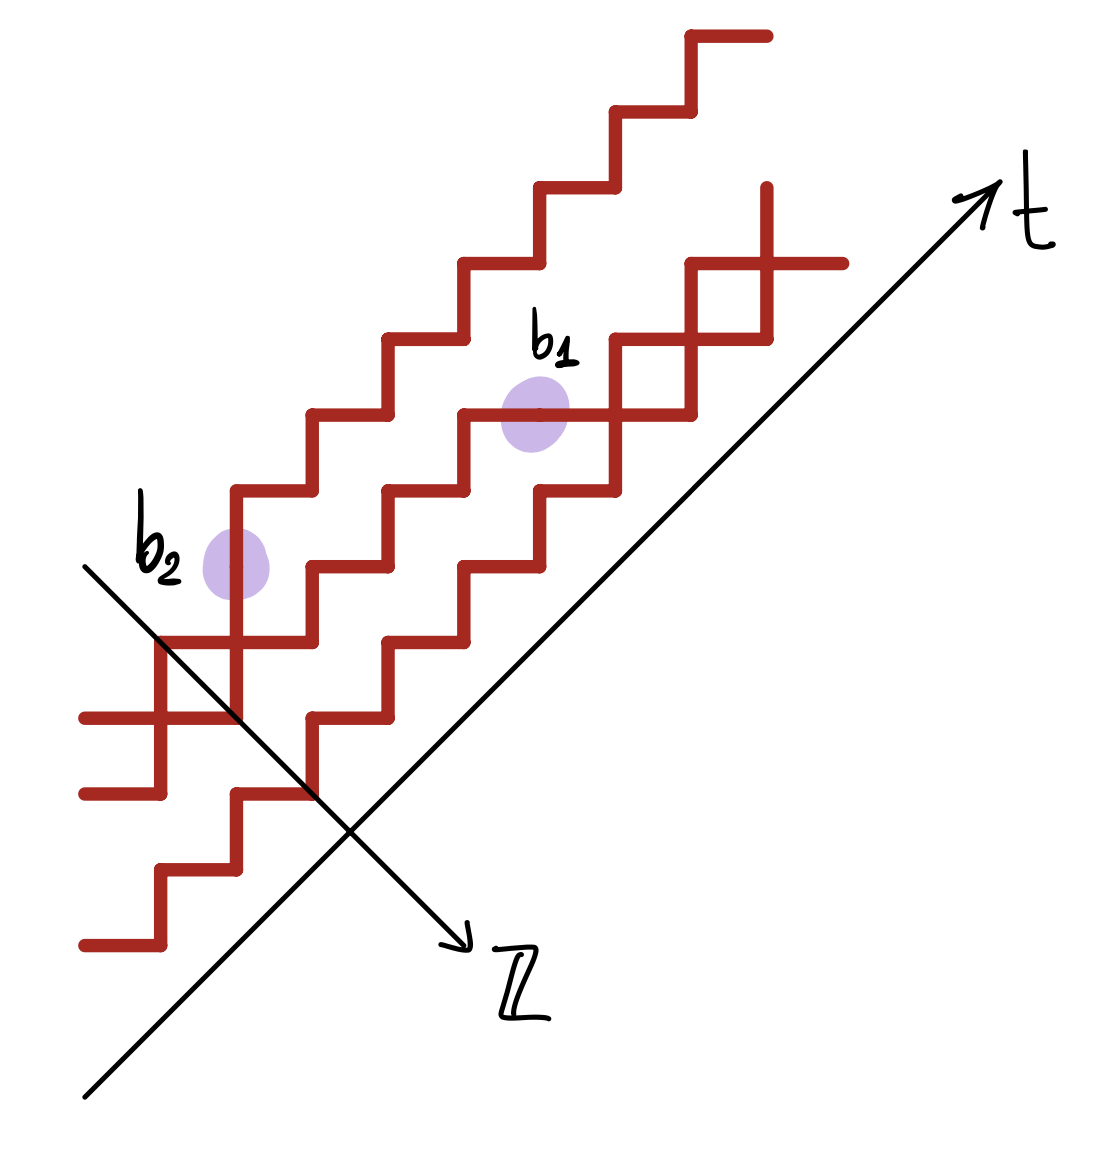
\includegraphics[width=.4\textwidth]{./images/staircase_s6v.png}
\end{equation*}
In this picture, we highlighted the two occasional moves, first ``up'' with probability $b_2$,
and second ``down'' with probability $b_1$.
In the Poisson type scaling limit
when the discrete diagonal time becomes continuous, 
the staircases may be mapped to interacting particles
on the line:
\begin{equation*}
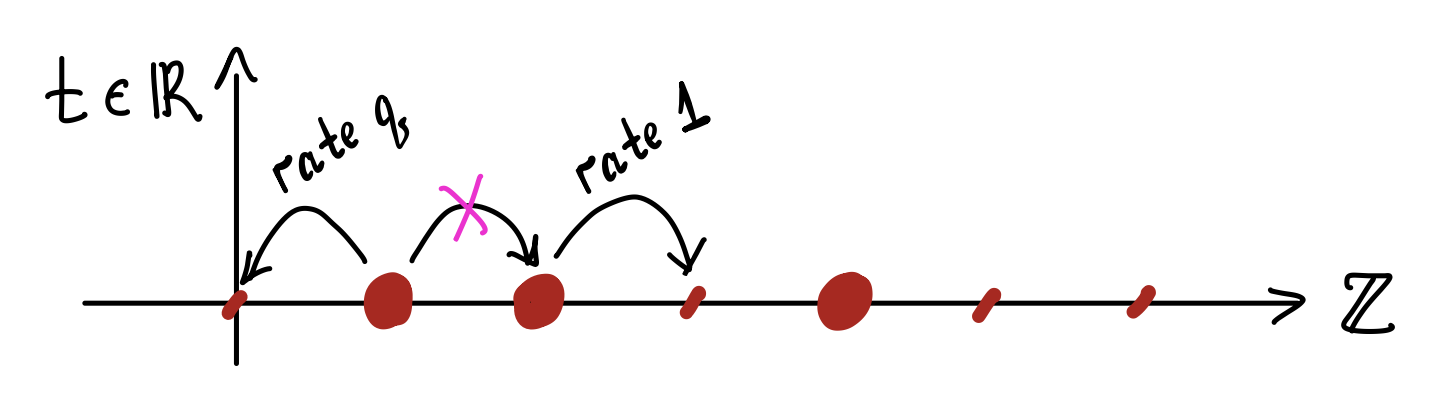
\includegraphics[width=.6\textwidth]{./images/ASEP.png}
\end{equation*}
The motion of the particles is as follows. In continuous time, each particle
has two independent exponential clocks
with rates $1$ and $q$. Clocks of different particles are independent
from each other. By ``exponential clocks of rate $\lambda$'' we mean a 
clocks which rings after an exponential random time $T$ with 
$\mathop{\mathrm{Prob}}(T>s)=e^{-\lambda s}$. Due to the memorylessness
of the exponential distribution, the 
ringing of one clock does not affect all other clocks.
When a clock of rate $q$ or $1$ 
at a particle rings,
it jumps left or right by one, respectively, under the condition that the destination is not occupied.
If the destination is occupied, the jump is suppressed.

This particle system (Markov process on particle
configurations on $\mathbb{Z}$) is called the Asymmetric Simple Exclusion Process, or \emph{ASEP}, for short.
It was introduced over 50 years ago in biology
\cite{macdonald1968bioASEP},
\cite{MacdonaldGibbsASEP1969}
and probability \cite{Spitzer1970}.

In our limit from the stochastic six vertex model, the initial condition
for ASEP is the \emph{step initial condition}, under which all
negative sites of $\mathbb{Z}$ are occupied.
However, 
ASEP can start from an arbitrary particle configuration on $\mathbb{Z}$, and the existence of the 
process can be established using Harris' graphical construction
\cite{Harris1978}.
In the particular case $q=0$, ASEP turns into TASEP (Totally Asymmetric Simple Exclusion Process),
in which particles jump only to the right.

\subsubsection{PushTASEP limit}
\label{subsub:PushTASEP_limit}

Let us keep the infinite domain wall boundary condition in the stochastic six vertex model.
In another Poisson type limit as $c_1\to0$,
the up-right paths become very long and horizontal.
For simplicity, let us first assume that also $b_2=0$.
Treating the horizontal axis as the new time, and 
rescaling this time from discrete to continuous
by the factor of $c_1^{-1}$ leads to a particle system
which is known as PushTASEP (Pushing Totally Asymmetric Simple Exclusion Process)
or long-range TASEP. 
PushTASEP is a very close relative of TASEP. It was introduced in
\cite{Spitzer1970} and studied in a number of papers, including
\cite{derrida1991dynamics},
\cite{diekerWarren2008determinantal},
\cite{BorFerr08push}.

In the PushTASEP limit of the stochastic six vertex model, particles live on $\mathbb{Z}_{\ge0}$ 
(which we draw vertical) and jump up in continuous time. 
Each particle has an independent exponential clock of rate $1$. 
When the clock rings, the particle jumps up by $1$, and pushes up by $1$ any particle that is in the way:
\begin{equation*}
	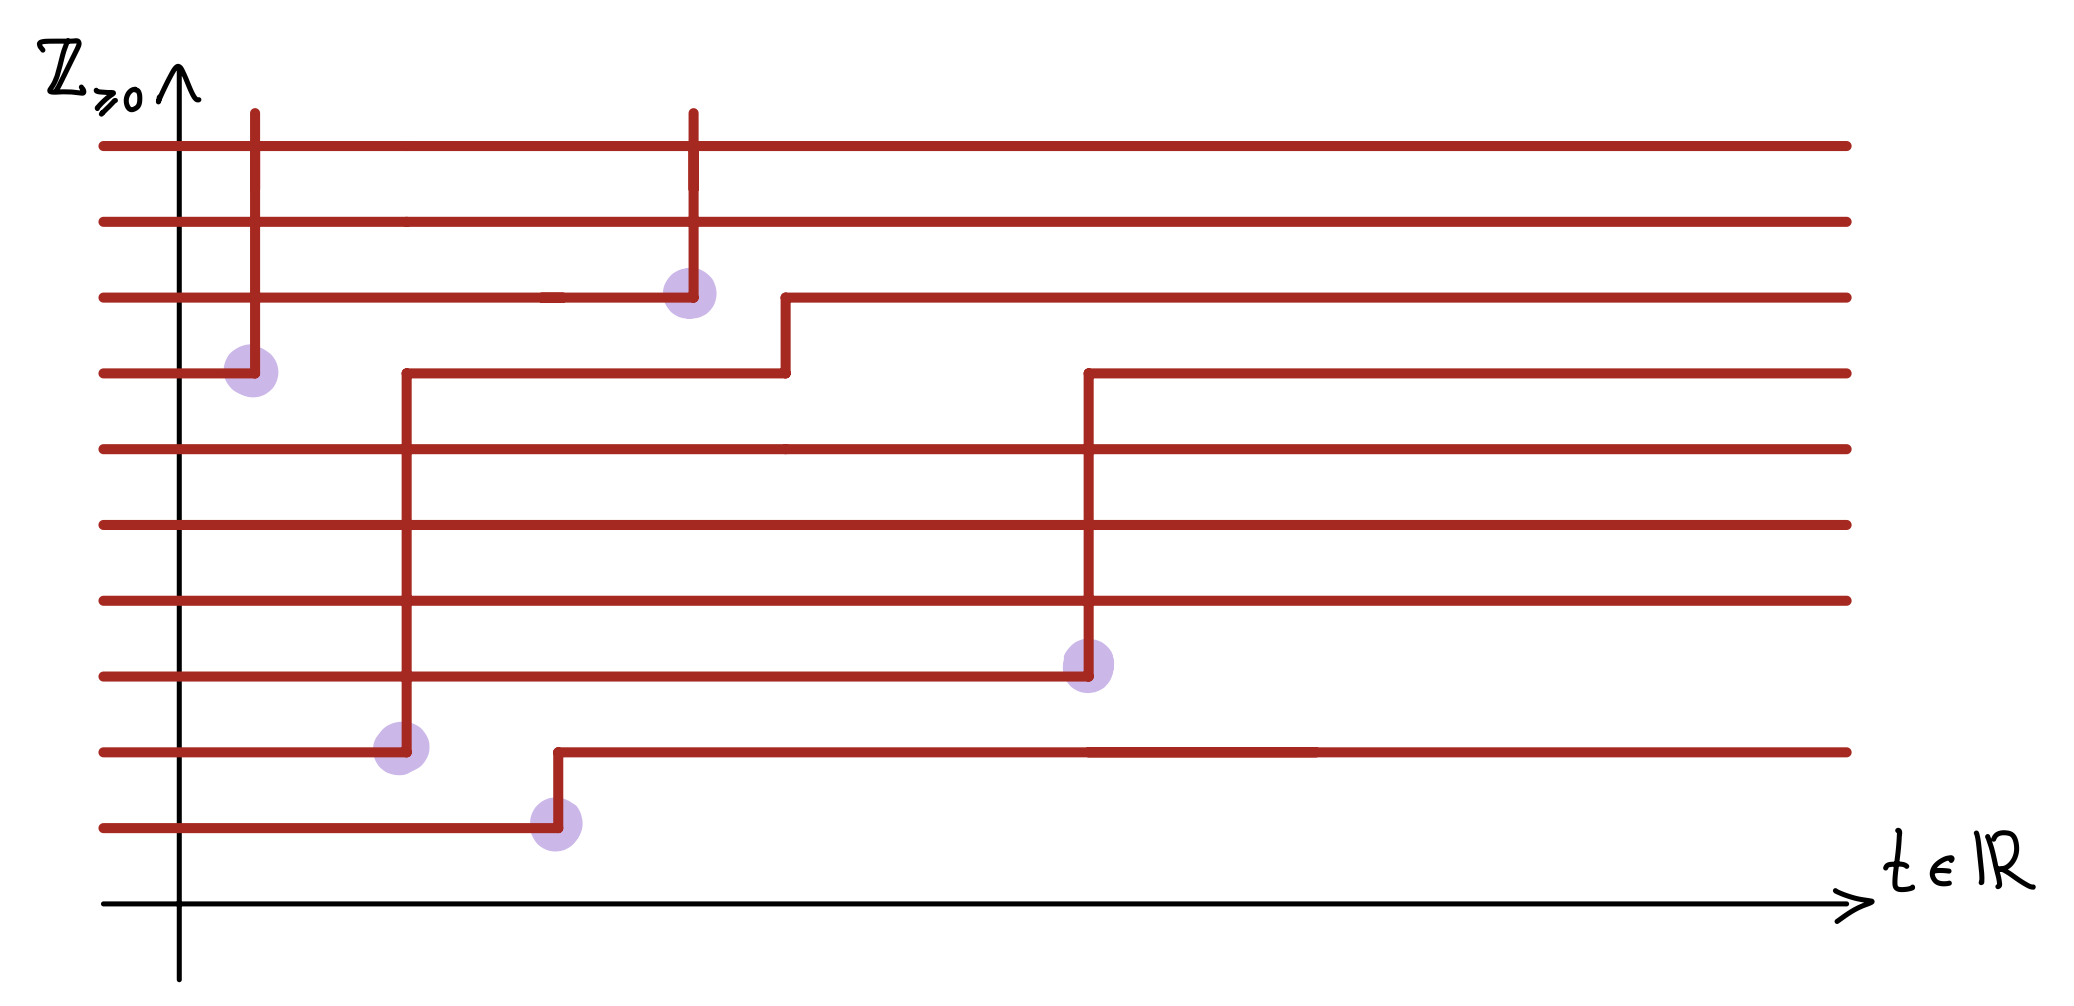
\includegraphics[width=.7\textwidth]{./images/PushTASEP.png}
\end{equation*}
Here we highlighted the rare events which occur with probability $c_1\to1$.

\begin{remark}
	\label{rmk:PushTASEP_inf_jumps}
	For the PushTASEP coming from the infinite domain wall boundary condition, in any finite
	time interval $[0,t)$, infinitely many particles get pushed up to infinity and leave the system. 
	This infinity of jumps in a finite time does not create problems, since 
	the marginal evolution of the PushTASEP restricted to $\left\{ 0,1,2,\ldots,K  \right\}\subset\mathbb{Z}_{\ge0}$
	for any $K\ge1$ is independent of the rest of the system. Therefore, we can define the 
	evolution of the PushTASEP on the whole lattice $\mathbb{Z}_{\ge0}$
	by Kolmogorov extension.
\end{remark}

If we did not set $b_2=0$ in the PushTASEP limit, 
we would get a one-parameter deformation of PushTASEP
which is known as the \emph{Hall-Littlewood PushTASEP}
\cite{BorodinBufetovWheeler2016},
\cite{Ghosal2017KPZ}.
In this deformed process, each jumping particle first jumps up by $1$, but then can 
continue moving up, with probability $q\in[0,1)$ per each extra step,
as long as there are no other particles in the way. When 
there is a particle in the way, the moving particle 
stops, but the next particle is activated, and will continue 
jumping up according to the same mechanism.
Here, as before, $q=b_2/b_1$, and recall that $b_1\to1$.

\begin{exercise}
	Prove the claims made in \Cref{rmk:PushTASEP_inf_jumps}, and 
	extend them to the Hall-Littlewood PushTASEP. Is the marginal Markov
	structure of the PushTASEP preserved under the deformation?
\end{exercise}


\subsection{Gibbs measures from the stochastic six vertex model}
\label{sub:Gibbs_s6v}

The stochastic six vertex model Gibbs property
depending on two parameters $(b_1,b_2)$
seems much more restrictive than the 
Gibbs property of the general six vertex model
with all six parameters
$(a_1,a_2,b_1,b_2,c_1,c_2)$, 
see \eqref{eq:6v_weights_picture}.
However, by renormalizing the vertex weights
in a finite region $\Lambda\subset\mathbb{Z}^{2}$,
we may reduce a rather general six vertex model Gibbs property 
(namely, the symmetric, ferroelectric one)
to the 
stochastic one.
This result is due to Aggarwal \cite[Appendix A.1]{Amol2016Stationary}
using some of the observations from \cite{BorodinBufetov2015}.
For convenience, we reproduce the full proof here.

\begin{proposition}
	\label{prop:Aggarwal_lemma_Gibbs_property}
	Let $a_1=a_2=\mathscr{A}$, $b_1=b_2=\mathscr{B}$, and $c_1=c_2=\mathscr{C}$, where
	$\mathscr{A},\mathscr{B},\mathscr{C}\ge0$ satisfy the ferroelectric condition
	\begin{equation*}
		\Delta=\frac{\mathscr{A}^2+\mathscr{B}^2-\mathscr{C}^2}{2\mathscr{A}\mathscr{B}}>1
	\end{equation*}
	and $\mathscr{A}>\mathscr{B}$.
	Then, in any finite region $\Lambda\subset\mathbb{Z}^{2}$ with fixed boundary 
	conditions on all sides, the Gibbs measure under the six vertex model
	with parameters $(a_1,a_2,b_1,b_2,c_1,c_2)$
	coincides with the Gibbs measure
	under the \emph{stochastic} six vertex model with parameters $(\tilde b_1,\tilde b_2)$,
	where 
	\begin{equation}
		\label{eq:Aggarwal_lemma_Gibbs_property_formulation}
		\tilde b_1=\frac{\mathscr{B}}{\mathscr{A}}\left( \Delta+\sqrt{\Delta^2-1} \right)
		,\qquad 
		\tilde b_2=\frac{\mathscr{B}}{\mathscr{A}}\left( \Delta-\sqrt{\Delta^2-1} \right).
	\end{equation}
\end{proposition}
The condition $\mathscr{A}>\mathscr{B}$ is not restrictive. Indeed, 
if $\mathscr{A}=\mathscr{B}$, we cannot have $\Delta>1$. 
If $\mathscr{A}<\mathscr{B}$, we can 
exchange $\mathscr{A}$ and $\mathscr{B}$ by
rotating the lattice clockwise by 90 degrees
and flipping the spins $\sigma_e\mapsto 1-\sigma_e$ for each horizontal edge $e$.
Thus, it suffices to assume $\mathscr{A}>\mathscr{B}$.

For $\mathscr{A}>\mathscr{B}$, the condition $\Delta>1$ is required
so that the resulting stochastic six vertex model
is an honest probability distribution with real nonnegative probability weights, 
that is, $\tilde b_1,\tilde b_2\in[0,1]$.
\begin{proof}[Proof of \Cref{prop:Aggarwal_lemma_Gibbs_property}]
	The argument relies on \emph{conservation laws} which hold in the finite region $\Lambda$
	with fixed boundary conditions.
	For each given configuration of up-right paths in $\Lambda$, 
	denote by 
	$\#_{a_1},\#_{a_2},\#_{b_1},\#_{b_2},\#_{c_1},\#_{c_2} $
	the number of vertices of the corresponding type in this configuration,
	see \eqref{eq:6v_weights_picture}.
	Then we have (where $const$ stand for quantities which depend only on $\Lambda$ and the
	fixed boundary conditions, but not on a particular configuration of up-right paths):
	\begin{enumerate}[$\bullet$]
		\item $\#_{a_1}+\#_{a_2}+\#_{b_1}+\#_{b_2}+\#_{c_1}+\#_{c_2}=const$, because this is the total number of
			vertices in $\Lambda$;
		\item 
			$\#_{a_2}+\#_{b_2}+\#_{c_1}=const$, because the total number of occupied vertical edges (i.e., with spin~$1$)
			is constant, and each vertical edge begins at a vertex of type $a_2$, $b_2$, or $c_1$;
		\item 
			$\#_{a_2}+\#_{b_1}+\#_{c_2}=const$, by similarly considering occupied horizontal edges;
		\item 
			$\#_{c_1}-\#_{c_2}=const$,
			see \Cref{exercise:six_Gibbs_2} below for details.
		\item 
			$\#_{b_1}-\#_{b_2}=const$, which follows from the previous three conservation laws.
	\end{enumerate}
	
	Using these conservation laws, one can check that the six vertex Gibbs measures
	with parameters $(a_1,a_2,b_1,b_2,c_1,c_2)$ and 
	the modified parameters
	$(w a_1,w a_2,wt^{-1}b_1,w t b_2,w\xi^{-1} c_1,w\xi c_2)$
	(where $w,t,\xi >0$ are arbitrary)
	are the same. Taking
	$a_1=a_2=\mathscr{A}$, $b_1=b_2=\mathscr{B}$, and $c_1=c_2=\mathscr{C}$, and
	\begin{equation*}
		w=\mathscr{A}^{-1},\qquad 
		t=\Delta+\sqrt{\Delta^2-1},\qquad 
		\xi=\frac{\mathscr{A}(1-\tilde b_2)}{\mathscr{C}}
		=
		\frac{\mathscr{A}-\mathscr{B}\Delta+\mathscr{B}\sqrt{\Delta^2-1}}{\mathscr{C}}
	\end{equation*}
	makes the 
	modified parameters
	of the Gibbs measure stochastic, namely,
	$(1,1,\tilde b_1,\tilde b_2,1-\tilde b_1,1-\tilde b_2)$. This completes the proof.
\end{proof}

\begin{exercise}
	\label{exercise:six_Gibbs}
			Verify the two claims made before the 
			proof of \Cref{prop:Aggarwal_lemma_Gibbs_property}.
\end{exercise}
\begin{exercise}
	\label{exercise:six_Gibbs_2}
	\begin{enumerate}[(a)]
		\item 
			Show the conservation law $\#_{c_1}-\#_{c_2}=const$.
			Argue as follows. First, show that any up-right path configuration
			in $\Lambda$ can be related to any other up-right configuration
			with the same boundary conditions
			by a sequence of local flips of the form:
			\begin{equation}
				\label{eq:Glauber_flips}
				\parbox{.7\textwidth}{
				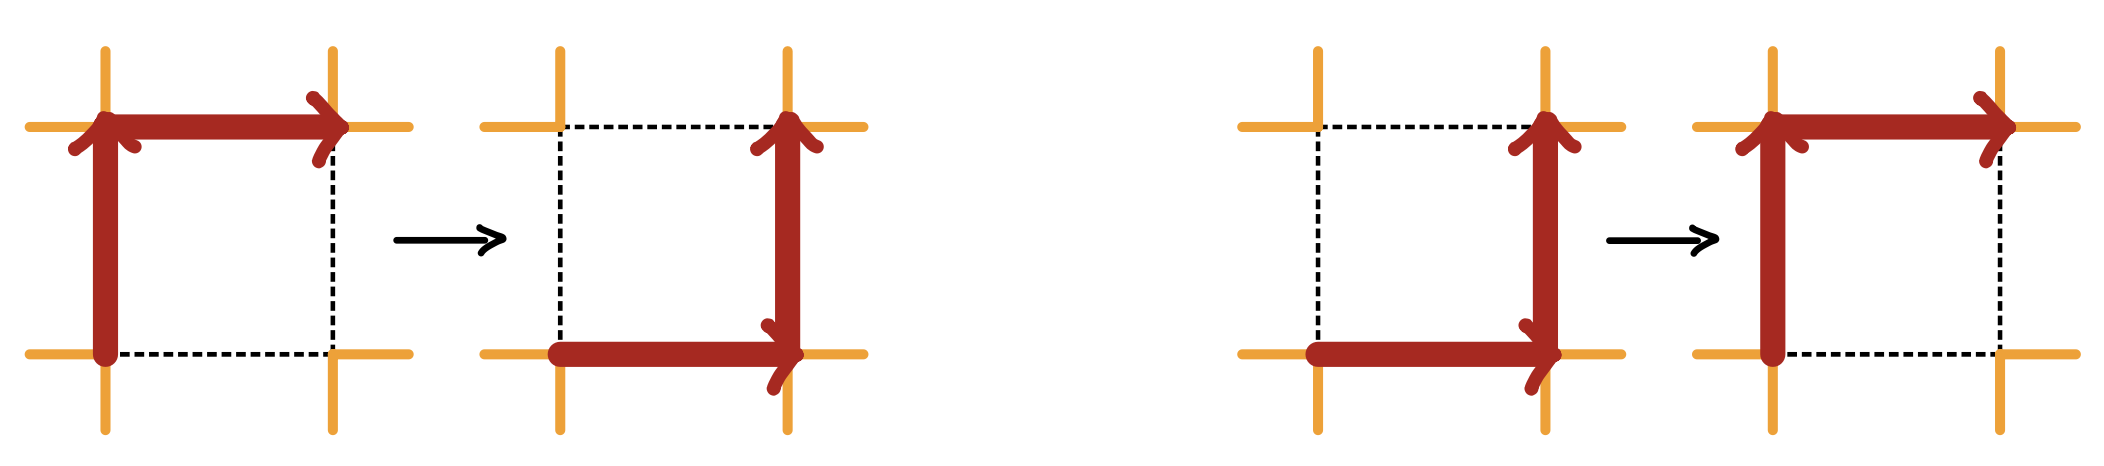
\includegraphics[width=.7\textwidth]{./images/Glauber_flips.png}}
			\end{equation}
			Here we change only the configuration 
			of occupied edges along a single lattice square, and do not change any other 
			parts of the configuration (which can be arbitrary outside this single square).
		\item 
			Show that under the flips \eqref{eq:Glauber_flips}, the numbers 
			$\#_{c_1}$ change $\#_{c_2}$ by the same amount, so that their
			difference stays constant.
	\end{enumerate}
\end{exercise}

By \Cref{prop:Aggarwal_lemma_Gibbs_property},
all possible Gibbs measures of the 
symmetric, ferroelectric six vertex model in a finite volume are 
obtained by running the stochastic six vertex Markov chain
with given initial conditions and conditioned on a given final configuration.
By taking limits, this observation allows to study pure states of 
symmetric, ferroelectric six vertex model by probabilistic techniques.
For example, this approach is employed by Aggarwal in
\cite{aggarwal2020nonexistence}.

\subsection{Basic coupling and colored (multispecies) models}
\label{sub:colored}

??? did not explain in the lecture

\begin{figure}[htpb]
	\centering
	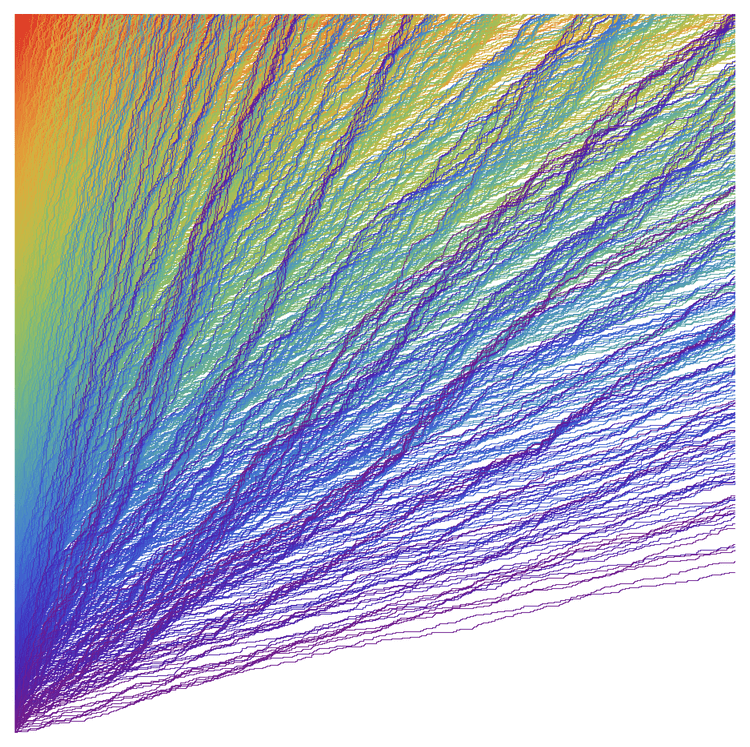
\includegraphics[width=.3\textwidth]{./images/CS6V.png}
	\quad
	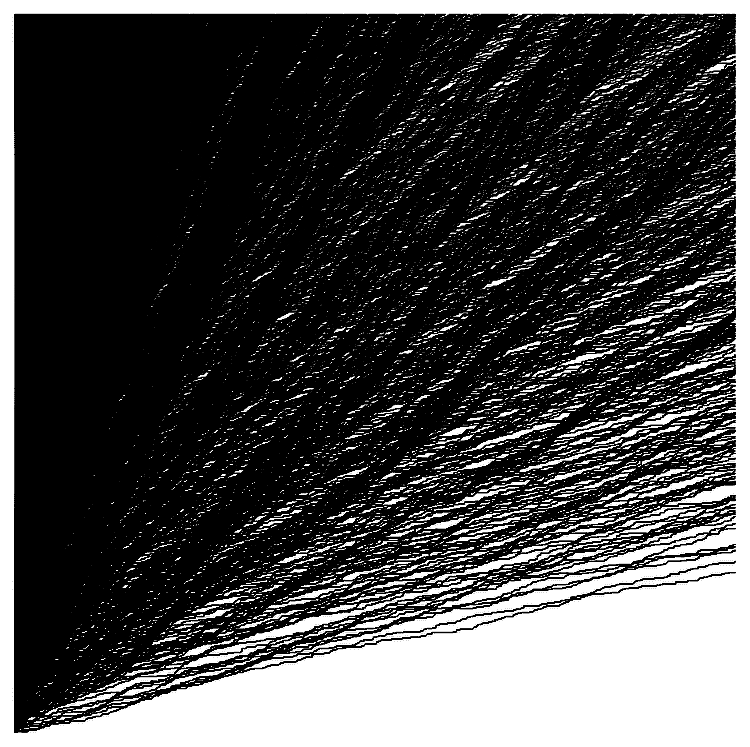
\includegraphics[width=.3\textwidth]{./images/S6V.png}
	\quad
	\raisebox{2pt}{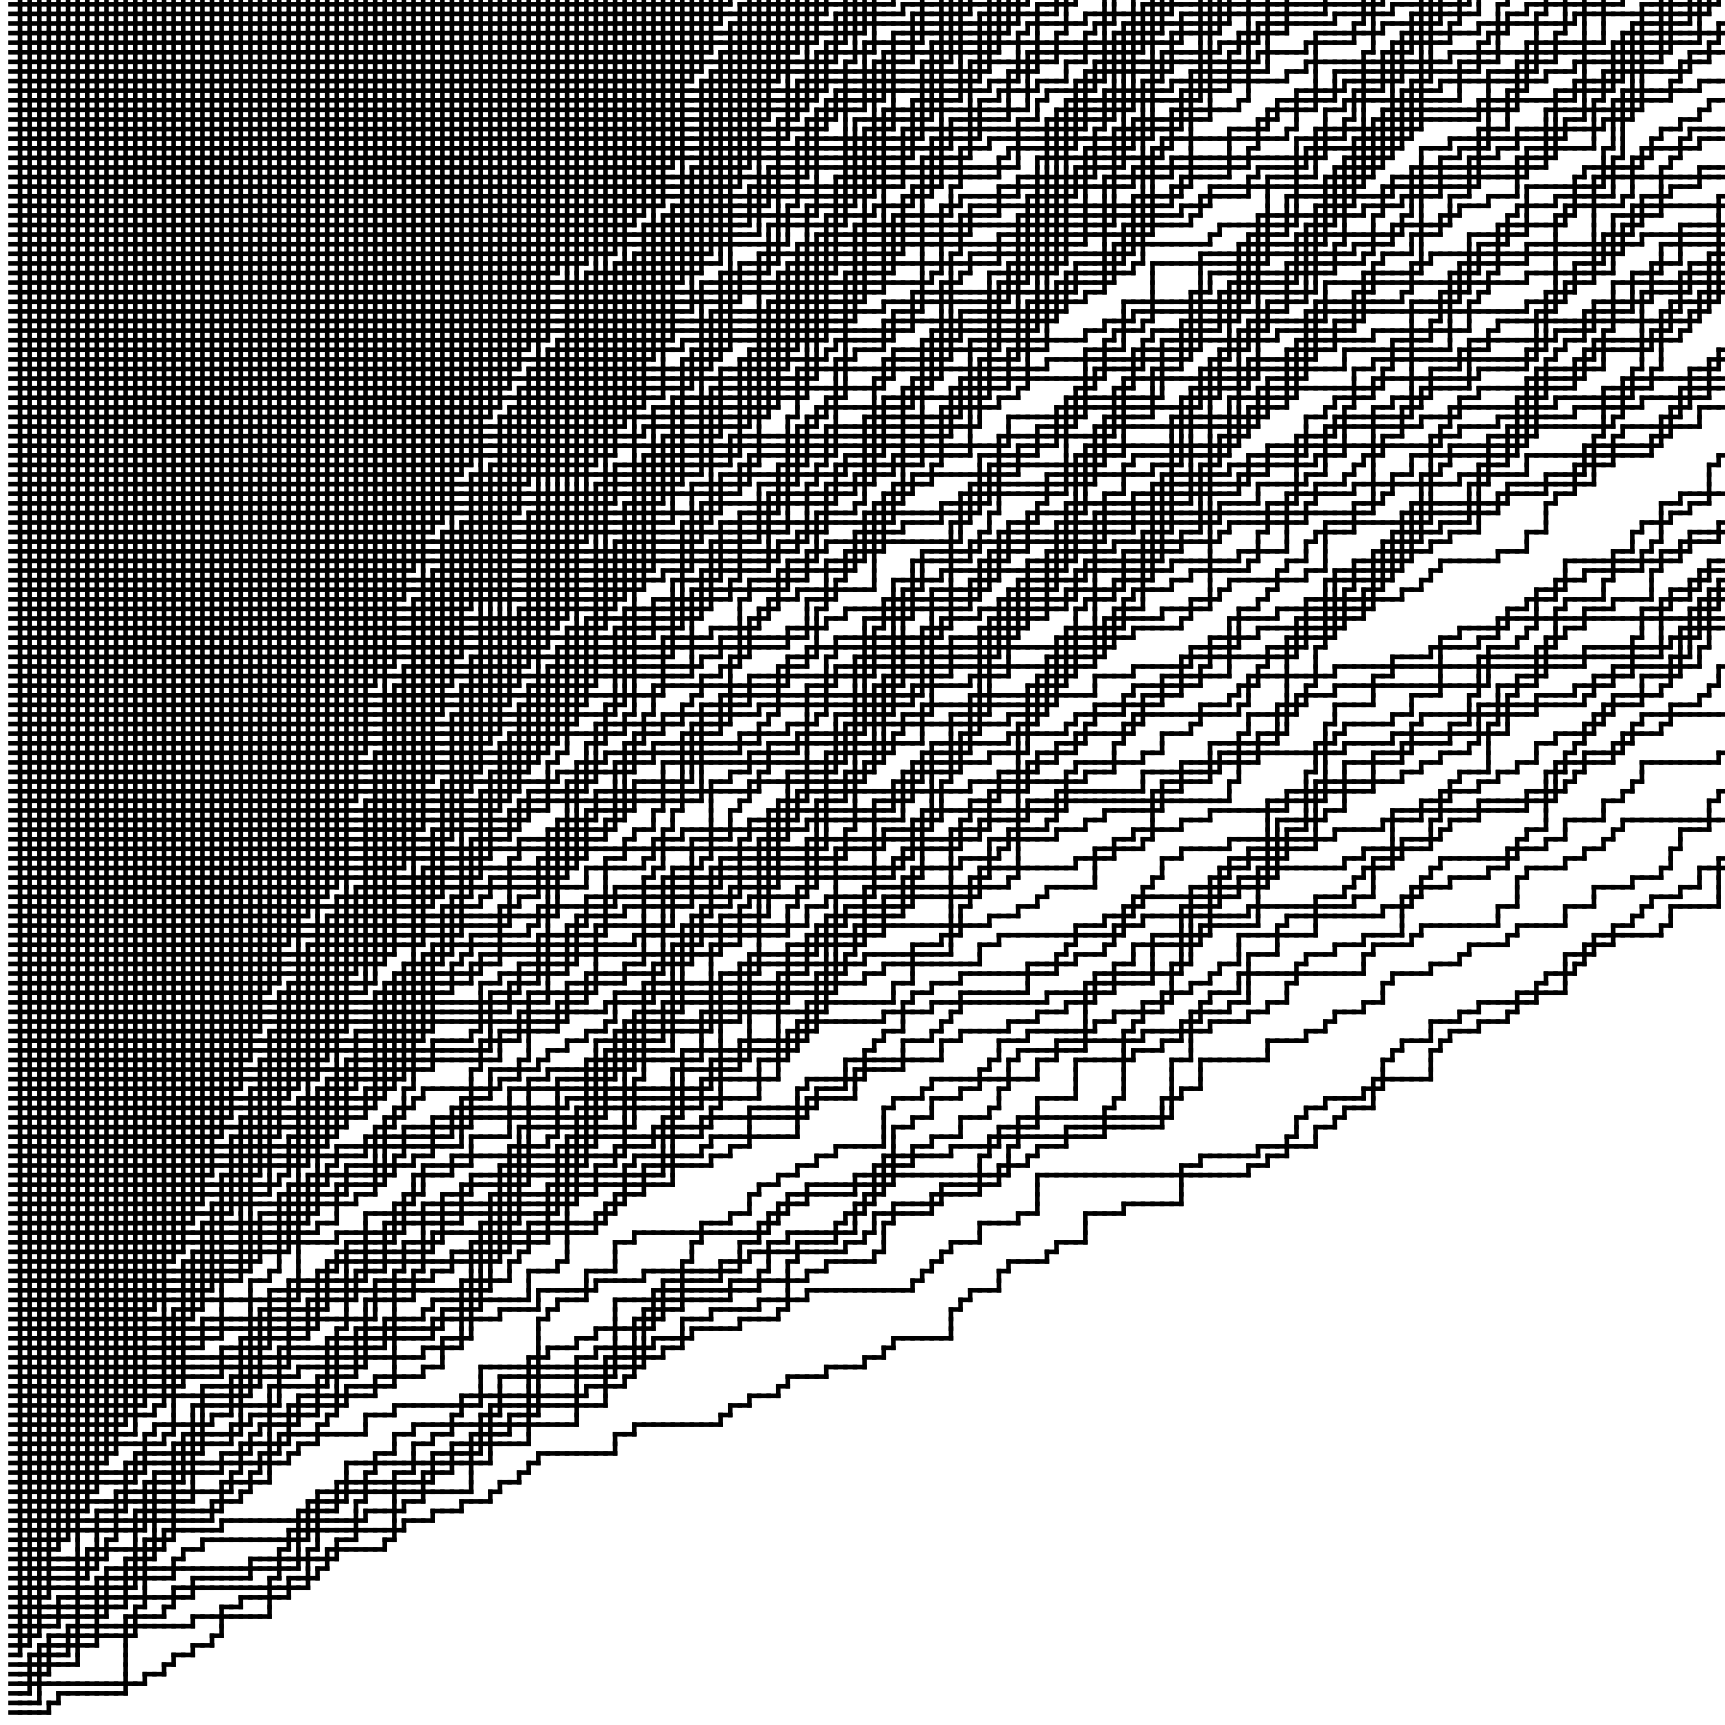
\includegraphics[width=.29\textwidth]{./images/stoch6v1.png}}
	\caption{Colored stochastic six vertex model, its monochrome version,
	and a smaller simulation of the monochrome six vertex model.}
	\label{fig:CS6V}
\end{figure}



\subsection{Stationary distributions and hydrodynamics}
\label{sub:hydrodynamic_analysis}




Bernoulli is Stationary; also for all the limits we had.

\begin{equation}
	\label{eq:Burgers_s6v}
\end{equation}

Limit shape check


\begin{exercise}
	For the infinite domain wall boundary condition,
	the limiting 
	density
	\begin{equation*}
		\rho(\mathsf{x},\mathsf{y})=-\partial_\mathsf{x} \mathfrak{h}(\mathsf{x},\mathsf{y}),
	\end{equation*}
	where $\mathfrak{h}$ is 
	given by \eqref{eq:limit_shape_height_function},
	is explicit. Check that this explicit density
	satisfies the Burgers type equation
	\eqref{eq:Burgers_s6v}.
\end{exercise}









\newpage
\section{Lecture II. Integrability}
\label{sec:integrability}





\newpage
\section{Lecture III. Asymptotics}
\label{sec:asymptotics}







\newpage
\bibliographystyle{alpha}
\bibliography{bib}

\medskip

\textsc{University of Virginia, Charlottesville, VA}

E-mail: \texttt{lenia.petrov@gmail.com}


\end{document}
